


\section{More Structure} 
\begin{frame}\frametitle{More Structure} 
\begin{itemize}
\item Classes
\item Classes: Behind the Scenes
\item Modules
\item Files
%\item File structure (require)
\end{itemize}
\end{frame}



\subsection{Classes}
\begin{frame}[fragile]\frametitle{Introduction}

\lstinputlisting[language=ruby]{code/thing.rb}
\pause

\begin{columns}[c] 

\begin{column}{5.5cm}

\begin{itemize}
\item getters/setters
\item instance variables
\end{itemize}

\end{column}

\begin{column}{5.5cm}

\begin{itemize}
\item default constructor
\end{itemize}

\end{column}

\end{columns}

\end{frame}



\begin{frame}[fragile]\frametitle{Introduction, cont.}

\lstinputlisting[language=ruby]{code/thing2.rb}
\pause

\begin{itemize}
\item \texttt{attr\_accessor}, \texttt{attr\_reader} and \texttt{attr\_writer}

\item constructors, parameters and default values
\end{itemize}

\end{frame}



\begin{frame}[fragile]\frametitle{Inheritance}
\lstinputlisting[language=ruby, firstline=1, lastline=12]{code/thing3.rb}

\begin{itemize}
\item proper method argument defaults
\end{itemize}
\end{frame}

\begin{frame}[fragile]\frametitle{Inheritance, cont.}
\lstinputlisting[language=ruby, firstline=14, firstnumber=14]{code/thing3.rb}

\begin{itemize}
\item single class inheritance
\item \texttt{super}
\end{itemize}
\end{frame}





\begin{frame}[fragile]\frametitle{Duck Typing}

\begin{columns}[c]

\begin{column}{5.5cm}

\begin{itemize}
\item Semantics are determined by an object's methods

\begin{itemize}
\item ...and not by its inheritance
\item ...or interfaces for other languages
\end{itemize}

\end{itemize}

\pause

\begin{quote}
``If it walks like a duck, and quacks like a duck, it is a duck.''
\end{quote}

\end{column}

\pause

\begin{column}{5.5cm}
\lstinputlisting[language=ruby]{code/duck_typing.rb}
\end{column}

\end{columns}

\end{frame}




\begin{frame}[fragile]\frametitle{Access Control}

\begin{columns}[c] 

\begin{column}{5.2cm}
\begin{lstlisting}[language=ruby]
class MyClass
  def method_one
  end
  
  protected
  def method_two
  end
  
  private
  def method_three
  end
  
  public
  def method_four
  end
end
\end{lstlisting}
\end{column}
\pause
\begin{column}{5.4cm}
\begin{lstlisting}[language=ruby]
class MyClass
  def method_one
  end
  
  def method_two
  end
  
  def method_three
  end
  
  def method_four
  end
  
  public    :method_one, 
            :method_four
  protected :method_two
  private   :method_three
end
\end{lstlisting}
\end{column}

\end{columns}

\end{frame}



\begin{frame}[fragile]\frametitle{Access Control, cont.}

\begin{itemize}
\item public
\begin{itemize}
\item can be accessed by any object
\end{itemize}

\item protected
\begin{itemize}
\item can be accessed from inside the defining class and its subclasses
\end{itemize}

\item private
\begin{itemize}
\item can be accessed only from inside the defining class
\end{itemize}

%http://stackoverflow.com/questions/2131921/how-to-make-instance-variables-private-in-ruby
%\item \tiny not applicable for class methods
%http://madebydna.com/all/code/2011/06/24/eigenclasses-demystified.html

\end{itemize}

\end{frame}






\begin{frame}[fragile]\frametitle{Class variables, methods and inheritance}
\begin{columns}[c] 

\begin{column}{5.2cm}
\lstinputlisting[language=ruby, lastline=16]{code/class_variables.rb}
\end{column}
\pause
\begin{column}{5.5cm}
\lstinputlisting[language=ruby, firstline=18, firstnumber=18]{code/class_variables.rb}

\end{column}

\end{columns}

%\pause
%\begin{itemize}
%\item but we define a class variable in \texttt{Treasure} it would not exist in \texttt{Thing}
%\end{itemize}

\end{frame}






\begin{frame}[fragile]\frametitle{Constants and scope resolution operator}
\lstinputlisting[language=ruby]{code/circle.rb}
\end{frame}






\begin{frame}[fragile]\frametitle{Partial Classes}

\begin{columns}[c] 

\begin{column}{5.5cm}
\begin{lstlisting}[language=bash]
class Dog
  def bark
    puts( "woof" )
  end
end

class Dog
  def bite
    puts( "yum" )
  end
end

\end{lstlisting}
\end{column}
\pause
\begin{column}{5.5cm}

\begin{itemize}
\item classes can be reopened
\item ...and new methods added
\item this applies to all classes!
\end{itemize}

\end{column}

\end{columns}

\end{frame}






\subsection{Classes: Behind the Scenes}
\begin{frame}[fragile]\frametitle{Introduction}


\begin{columns}[c] 

\begin{column}{4cm}
\begin{itemize}

\item Everything is an object
\item Every object has a class

\end{itemize}
\end{column}


\begin{column}{7cm}
\lstinputlisting[language=ruby]{code/person.rb}
\end{column}

\end{columns}

\end{frame}




\begin{frame}[fragile]\frametitle{Method lookup path: object}

\begin{columns}[c] 

\begin{column}{7.4cm}
\begin{lstlisting}[language=bash, escapechar={^}]
irb(main):005:0> aragorn = Person.new
=> #<Person:0x0000000285c3a0>  ^\pause^
irb(main):006:0> aragorn.class
=> Person                      ^\pause^
irb(main):007:0> Person.superclass
=> Object                      ^\pause^
irb(main):008:0> Object.superclass
=> BasicObject                 ^\pause^
irb(main):009:0> BasicObject.superclass
=> nil
\end{lstlisting}
\end{column}
\pause

\begin{column}{3.9cm}
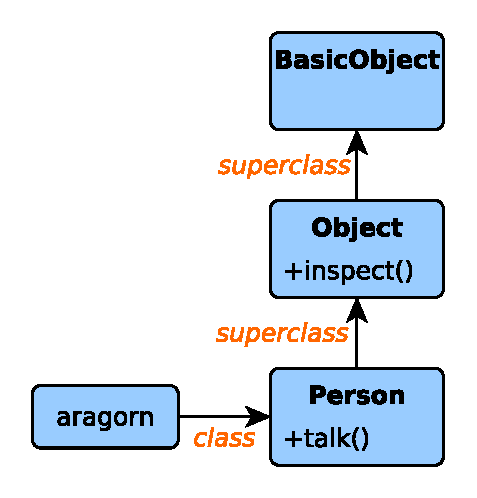
\includegraphics[scale=0.55]{diagrams/object_lookup_path.pdf}
\end{column}

\end{columns}

\end{frame}





\begin{frame}[fragile]\frametitle{Method lookup path: class object}

\begin{columns}[c] 

\begin{column}{7.4cm}

\begin{itemize}
\item A class is also an object!
\end{itemize}

\pause

\begin{lstlisting}[language=bash, escapechar={^}]
irb(main):005:0> aragorn = Person.new
=> #<Person:0x0000000285c3a0>
irb(main):006:0> aragorn.class
=> Person                           ^\pause^
irb(main):007:0> Person.class
=> Class                            ^\pause^
irb(main):008:0> Class.superclass
=> Module                           ^\pause^
irb(main):009:0> Module.superclass
=> Object                           ^\pause^
irb(main):010:0> Object.superclass 
=> BasicObject
\end{lstlisting}

\end{column}
\pause

\begin{column}{3.9cm}
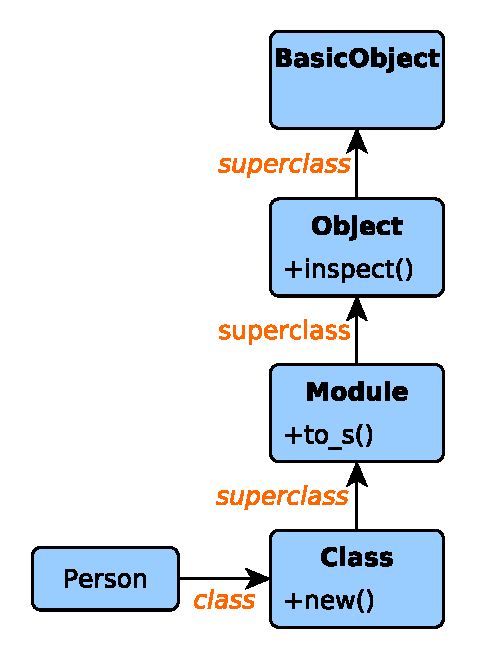
\includegraphics[scale=0.55]{diagrams/class_object_lookup_path.pdf}
\end{column}

\end{columns}

\end{frame}




\begin{frame}[fragile]\frametitle{Singleton Methods}

\begin{itemize}
\item A class defines the behaviour of their instances
\item Behaviour of person instances is placed in the Person class
\item Ruby allows unique behaviour to individual objects!
\end{itemize}

\pause
\lstinputlisting[language=ruby]{code/singleton_methods.rb}

\end{frame}




\begin{frame}[fragile]\frametitle{Eigenclasses (singleton classes, metaclasses, ghost classes)}

\begin{columns}[c] 

\begin{column}{5.5cm}
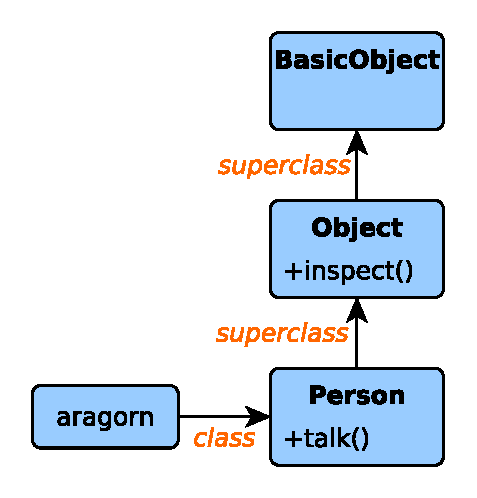
\includegraphics[scale=0.55]{diagrams/object_lookup_path.pdf}

\begin{itemize}
\item \alt<1>{Where is \texttt{aka}?}{There it is!}
\end{itemize}
\end{column}

\pause

\begin{column}{5.5cm}
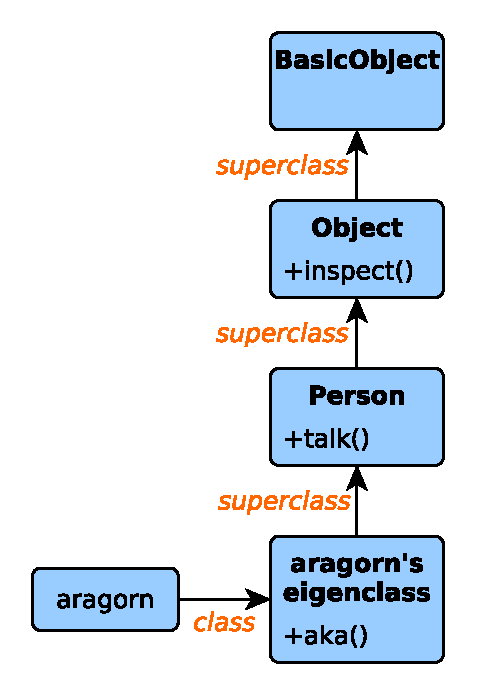
\includegraphics[scale=0.55]{diagrams/object_lookup_path2.pdf}
\end{column}

\end{columns}

\end{frame}




\begin{frame}[fragile]\frametitle{Eigenclasses and the \texttt{class <<} syntax}

\begin{columns}[c] 

\begin{column}{5.5cm}

\begin{itemize}
\item "one's very own" class
\item anonymous class
\item<3-> The \texttt{class <<} syntax opens the eigenclass of whatever object you pass to it
\end{itemize}

\end{column}

\pause

\begin{column}{5.5cm}

\lstinputlisting[language=ruby, firstline=4, lastline=6]{code/singleton_methods.rb}

\pause

\begin{lstlisting}[language=ruby, escapechar={^}]
class << aragorn
  def aka
    "Strider"
  end
end
\end{lstlisting}

\end{column}

\end{columns}

\end{frame}





\begin{frame}[fragile]\frametitle{Class Methods, revisited}

\begin{itemize}
\item classes are also objects, so
\begin{itemize}
\item ...they can have singleton methods 
\end{itemize}   \pause
\item In fact, what we call class methods are singleton methods for classes!
\end{itemize}

\pause

\begin{columns}[c] 

\begin{column}{5.5cm}

\begin{lstlisting}[language=ruby, escapechar={^}]
def Person.closest_dna
  "chimpanzee"
end
\end{lstlisting}
\pause
\begin{lstlisting}[language=ruby, escapechar={^}]
class Person
  def self.closest_dna
    "chimpanzee"
  end
end
\end{lstlisting}


\end{column}

\pause

\begin{column}{5.5cm}

\begin{lstlisting}[language=ruby, escapechar={^}]
class << Person
  def closest_dna
    "chimpanzee"
  end
end
\end{lstlisting}
\pause
\begin{lstlisting}[language=ruby, escapechar={^}]
class Person
  class << self
    def closest_dna
      "chimpanzee"
    end
  end
end
\end{lstlisting}

\end{column}

\end{columns}

\end{frame}




\begin{frame}\frametitle{Complete lookup path}
\begin{center}
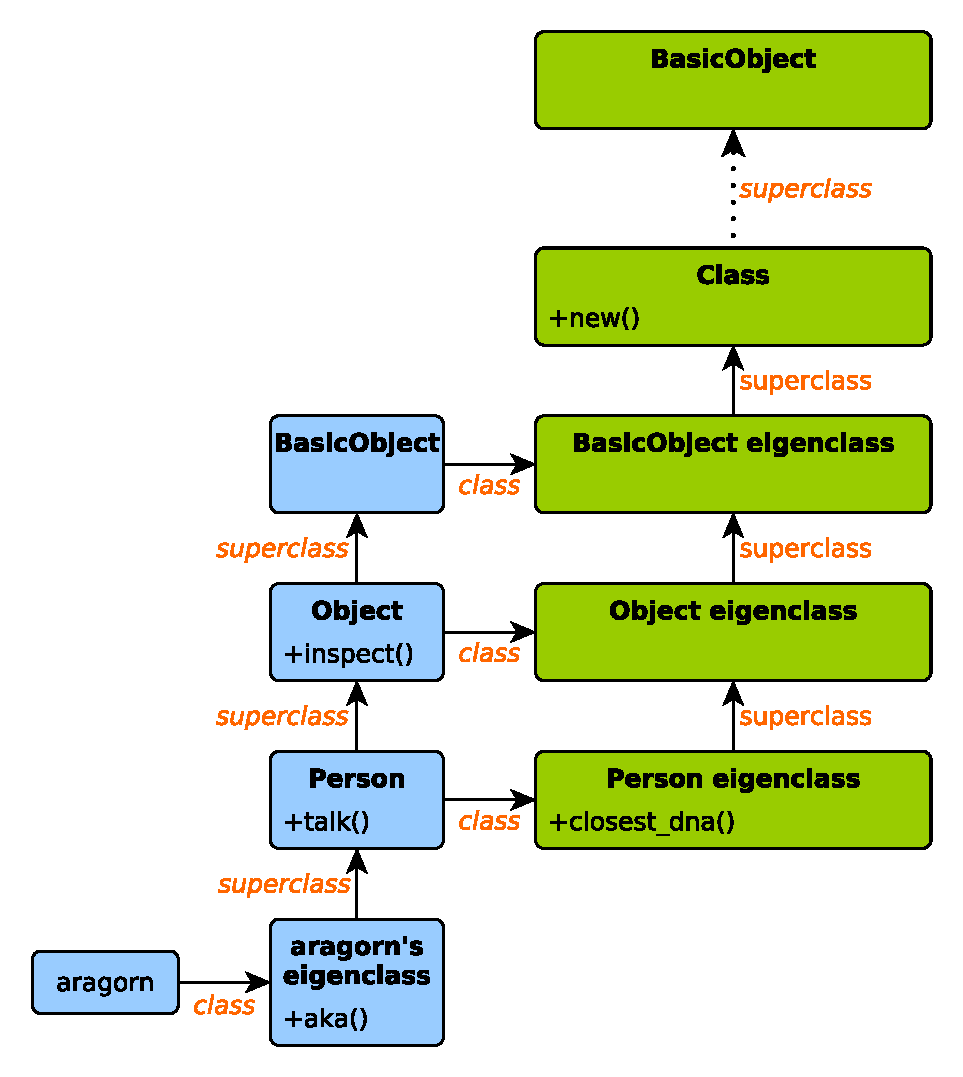
\includegraphics[scale=0.42]{diagrams/complete_lookup_path.pdf}
\end{center}
\end{frame}




\subsection{Modules}
\begin{frame}[fragile]\frametitle{Modules}

\begin{itemize}

\item A way of grouping together methods, classes and constants

\begin{itemize}
\item namespaces
\end{itemize}

\end{itemize}

\pause

\begin{columns}[c]

\begin{column}{5.3cm}
\begin{lstlisting}[language=bash, escapechar={^}]
irb:001> Math.sqrt(9)
 => 3.0                  ^\pause^
irb:002> Math::PI
 => 3.141592653589793    ^\pause^
irb:003> include Math
 => Object               ^\pause^
irb:004> sqrt(5)
 => 2.23606797749979     ^\pause^
irb:005> PI
 => 3.141592653589793 
\end{lstlisting}
\end{column}

\pause

\begin{column}{5.3cm}
\lstinputlisting[language=ruby]{code/module_trig.rb}
\end{column}

\end{columns}

\end{frame}





\begin{frame}[fragile]\frametitle{Modules, cont.}

\begin{itemize}

\item A way of adding extra functionality to classes

\begin{itemize}
\item mixins
\end{itemize}

\end{itemize}

\pause

\begin{columns}[c]

\begin{column}{5.4cm}
\lstinputlisting[language=ruby]{code/my_logger.rb}
\end{column}

\pause

\begin{column}{5.4cm}
\lstinputlisting[language=ruby]{code/person_mixins.rb}
\end{column}

\end{columns}

\end{frame}





\begin{frame}[fragile]\frametitle{Mixins, another example}

\begin{itemize}

\item Even more useful when mixin code interacts with class

\begin{itemize}
\item \texttt{Comparable} provides \texttt{<, <=, ==, >=, >, between?}
\item \texttt{Comparable} assumes class implements \texttt{<=>}
\end{itemize}

\end{itemize}

\pause

\begin{columns}[c]

\begin{column}{5.4cm}
\lstinputlisting[language=ruby, lastline=15]{code/person_comparable.rb}
\end{column}

\pause

\begin{column}{5.4cm}
\lstinputlisting[language=ruby, firstline=17, firstnumber=17]{code/person_comparable.rb}
\end{column}

\end{columns}

\end{frame}






\subsection{Files}
\begin{frame}[fragile]\frametitle{Files}

\begin{itemize}

\item Organise code into multiple files

\begin{itemize}
\item \texttt{load}
\item \texttt{require}
\item \texttt{require\_relative}
\end{itemize}

\end{itemize}

\pause

\begin{itemize}

\item Load path

\begin{itemize}
\item \texttt{\$LOAD\_PATH} or \texttt{\$:}
\end{itemize}

\end{itemize}


\end{frame}
%http://ruby.about.com/od/rubysbasicfeatures/ss/Load-Vs-Require.htm




\section{System Interaction} 
\begin{frame}\frametitle{System Interaction} 
\begin{itemize}
\item File System
\item Arguments
\item Environment
\item Shebang (hashbang)
\item Ruby Command Line
\end{itemize}
\end{frame}






\subsection{File System}
\begin{frame}[fragile]\frametitle{\texttt{File}}

\begin{columns}[c]

\begin{column}{7cm}

\begin{lstlisting}[language=ruby, escapechar={^}]
f = File.new("filename", "r")
f.each_line { |l| puts l }
f.close
\end{lstlisting}

\pause

\begin{lstlisting}[language=ruby, escapechar={^}]
File.open("filename", "r") do |f|
   f.each_line { |l| puts l }
end
\end{lstlisting}

\pause

\begin{lstlisting}[language=ruby, escapechar={^}]
IO.foreach("filename") { |l| puts l }
\end{lstlisting}

\end{column}

\pause

\begin{column}{4cm}
\begin{itemize}

\item \texttt{File}

\begin{itemize}
\item \texttt{.size}
\item \texttt{.exists?}
\item \texttt{.directory?}
\item \texttt{.writable?}
\item \texttt{.delete}
\item \texttt{.rename}
\item \texttt{.chown}
\item \texttt{.ctime}

\end{itemize}

\end{itemize}
\end{column}

\end{columns}

\end{frame}




\begin{frame}[fragile]\frametitle{\texttt{Dir}}

\begin{columns}[c]

\begin{column}{7cm}

\begin{lstlisting}[language=ruby, escapechar={^}]
Dir.foreach("/usr/bin") do |entry|
   puts entry
end
\end{lstlisting}

\pause

\begin{lstlisting}[language=ruby, escapechar={^}]
Dir.entries("/usr/bin").join(' ')
\end{lstlisting}

\pause

\begin{lstlisting}[language=ruby, escapechar={^}]
Dir["/usr/bin/*"]
\end{lstlisting}

\end{column}

\pause

\begin{column}{4cm}
\begin{itemize}

\item \texttt{Dir}

\begin{itemize}
\item \texttt{.chdir}
\item \texttt{.mkdir}
\item \texttt{.pwd}

\end{itemize}

\end{itemize}
\end{column}

\end{columns}

\end{frame}







\subsection{Arguments}
\begin{frame}[fragile]\frametitle{Arguments}

\begin{itemize}

\item Command-line arguments

\begin{itemize}
\item \texttt{ARGV} array
\item \texttt{ARGV.each \{ |a| puts a \}}
\end{itemize}

\item Check \texttt{optparse} from standard library

\end{itemize}

\end{frame}




\subsection{Environment}
\begin{frame}[fragile]\frametitle{Environment}

\begin{itemize}

\item Reading OS's environment variables

\begin{itemize}
\item \texttt{ENV} hash
\item \texttt{ENV.each \{ |k,v| puts "\#\{k\}=\#\{v\}" \} }
\end{itemize}

\end{itemize}

\end{frame}




\subsection{Shebang (hashbang)}
\begin{frame}[fragile]\frametitle{Shebang (hashbang)}
\begin{lstlisting}[language=ruby, escapechar={^}]
#!/usr/bin/env ruby

puts "Hello World!"
\end{lstlisting}
\pause
\begin{lstlisting}[language=bash, escapechar={^}]
$ chmod 755 file.rb
$ ./file.rb
Hello World
$
\end{lstlisting}
\end{frame}





\subsection{Ruby Command Line}
\begin{frame}[fragile]\frametitle{Ruby Command Line}

\begin{itemize}

\item Command line options

\begin{itemize}
\item \texttt{-v}
\pause
\item \texttt{-e}
\begin{itemize}
\item \lstinline!$ ruby -e 'puts "Hi"'!
\end{itemize}
\pause
\item \texttt{-n}
\begin{itemize}
\item \texttt{while gets; ... end}
\item \lstinline!$ echo -e "foo\nbar" | ruby -ne 'puts $_'!
\end{itemize}
\pause
\item \texttt{-p}
\begin{itemize}
\item \texttt{operates on \texttt{\$\_}} and writes it at every iteration
\item \lstinline!$ echo -e "foo\nbar" | ruby -pe 'chomp'!
\end{itemize}

\end{itemize}

\end{itemize}

\end{frame}






\section{Miscellaneous} 
\begin{frame}\frametitle{Miscellaneous} 
\begin{itemize}
\item Regular Expressions
\item Web Services
\item Concurrency: a bird's eye view
\item Metaprogramming: a bird's eye view
\end{itemize}
\end{frame}




\subsection{Regular Expressions}
\begin{frame}[fragile]\frametitle{Regular Expressions}

\begin{itemize}

\item A pattern that can be matched against a string

\begin{itemize}
\item \texttt{r = Regexp.new("pattern")}
\pause
\item \texttt{r = /pattern/}
\pause
\item \texttt{r = \%r\{pattern\}}
\pause
\item Operators: \texttt{=\~} and \texttt{!\~}
\end{itemize}

\end{itemize}

\pause

\begin{lstlisting}[language=ruby, escapechar={^}]
/lo/ =~ "hello"                         # => 3     ^\pause^
"hello" =~ /lo/                         # => 3     ^\pause^
"hello" =~ /hi/                         # => nil   ^\pause^
m = /ll/.match("hello")                 # => #<MatchData "ll"> ^\pause^
"#{m.pre_match}->#{m[0]}<-#{m.post_match}" 
# => "he->ll<-o" ^\pause^

if "hello" =~ /hi/
  # ..
end
\end{lstlisting}

\end{frame}




\begin{frame}[fragile]\frametitle{Regular Expressions, cont.}

\begin{itemize}

\item All characters match themselves except:

\begin{itemize}
\item \lstinline!. | ( ) [ ] { } + \ ^ $ * ?!
\end{itemize}

\end{itemize}

\pause

\begin{lstlisting}[language=ruby, escapechar={!}]
"hello" =~ /^el/                        # => nil !\pause!
"hello " =~ /lo$/                       # => nil !\pause!
"hello " =~ /[aeiou]/                   # => 1   !\pause!
"hello world" =~ /\s/                   # => 5   !\pause!
"hello world" =~ /\s[[:digit:]]/        # => nil !\pause!
"bat bit bot bet" =~ /(b.t )*/          # => 0   !\pause!
print $~                                # bat bit bot  => nil !\pause!
"bat bit bot bet" =~ /(b.t ){2}/        # => 0   !\pause!
print $~                                # bat bit => nil  !\pause!
"mississipi" =~ /(...)\1/i              # => 1   !\pause!
print $~                                # ississ => nil 
\end{lstlisting}

\end{frame}





\subsection{Web Services}
\begin{frame}[fragile]\frametitle{REST (\texttt{rest-client})}
\lstinputlisting[language=ruby]{code/rest_example.rb}
\end{frame}



\begin{frame}[fragile]\frametitle{SOA/SOAP (\texttt{savon} -- v2)}
\lstinputlisting[language=ruby]{code/soap_example.rb}
\end{frame}





\subsection{Concurrency: a bird's eye view}
\begin{frame}\frametitle{Concurrency: a bird's eye view}

\begin{itemize}[<+->]

\item Processes

\item Threads
\begin{itemize}

\item green threads (v1.8)
\item native threads (v1.9)
\begin{itemize}
\item GIL: data modified only by one thread at a time
\item ...but another thread could do I/O
\end{itemize}
\item JRuby, IronRuby, MacRuby, Rubinius, ...
\end{itemize}

\item Fibers
\begin{itemize}
\item \emph{lightweight} threads
\item ...but controlled by the developer
\end{itemize}

\end{itemize}

\end{frame}
%http://merbist.com/2011/02/22/concurrency-in-ruby-explained/



\subsection{Metaprogramming: a bird's eye view} 
\begin{frame}\frametitle{Metaprogramming: a bird's eye view} 
\begin{itemize}[<+->]

\item DSLs: writing code that writes code

\item Classes (and other language constructs) definition
\begin{itemize}
\item C, Pascal, ...
\item ...at compile time
\item Java, ...
\item ...at compile time and provides read access at runtime
\item Ruby
\item ...at compile time and provides read/write access at runtime
\end{itemize}

\end{itemize}
\end{frame}
